\documentclass[a4paper,10pt]{article}
\usepackage[utf8]{inputenc}

\usepackage[margin=25mm]{geometry}
\usepackage{times}
\usepackage{graphicx}

%opening
\title{TAKE-CV}
\author{Casey Kennington}

\begin{document}

\maketitle

\begin{abstract}
Description of the TAKE-CV data collection. 
\end{abstract}

\section{Summary}

The goal of this data collection is to form a corpus of referring expressions (\textsc{re}s) with a referred object called the \emph{target} and a potential object called the \emph{landmark} that is used to make a relative \textsc{re} (e.g., \emph{take the redd cross next to the green t}). 

\section{Materials}

\begin{itemize}
 \item microphone for the participant to record the \textsc{re}s
 \item camera for the objects which will be fed to OpenCV
 \item two monitors, one for the wizard and one for the participant to show which object is the target and landmark
 \item a PC to run the OpenCV/python scripts
 \item a PC to record the audio (could be the same as the above PC)
%  \item 
\end{itemize}

\section{Lab Layout}

See Figure \ref{layout}. The participant is seated near a table with the pento objects. A camera oriented so that it displays what the participant sees on the table (i.e., ``up'' in the video is the far side of the table from the perspective of the participant). A microphone is also near the participant to pick up speech and beeps. 

\begin{figure}
 \centering
      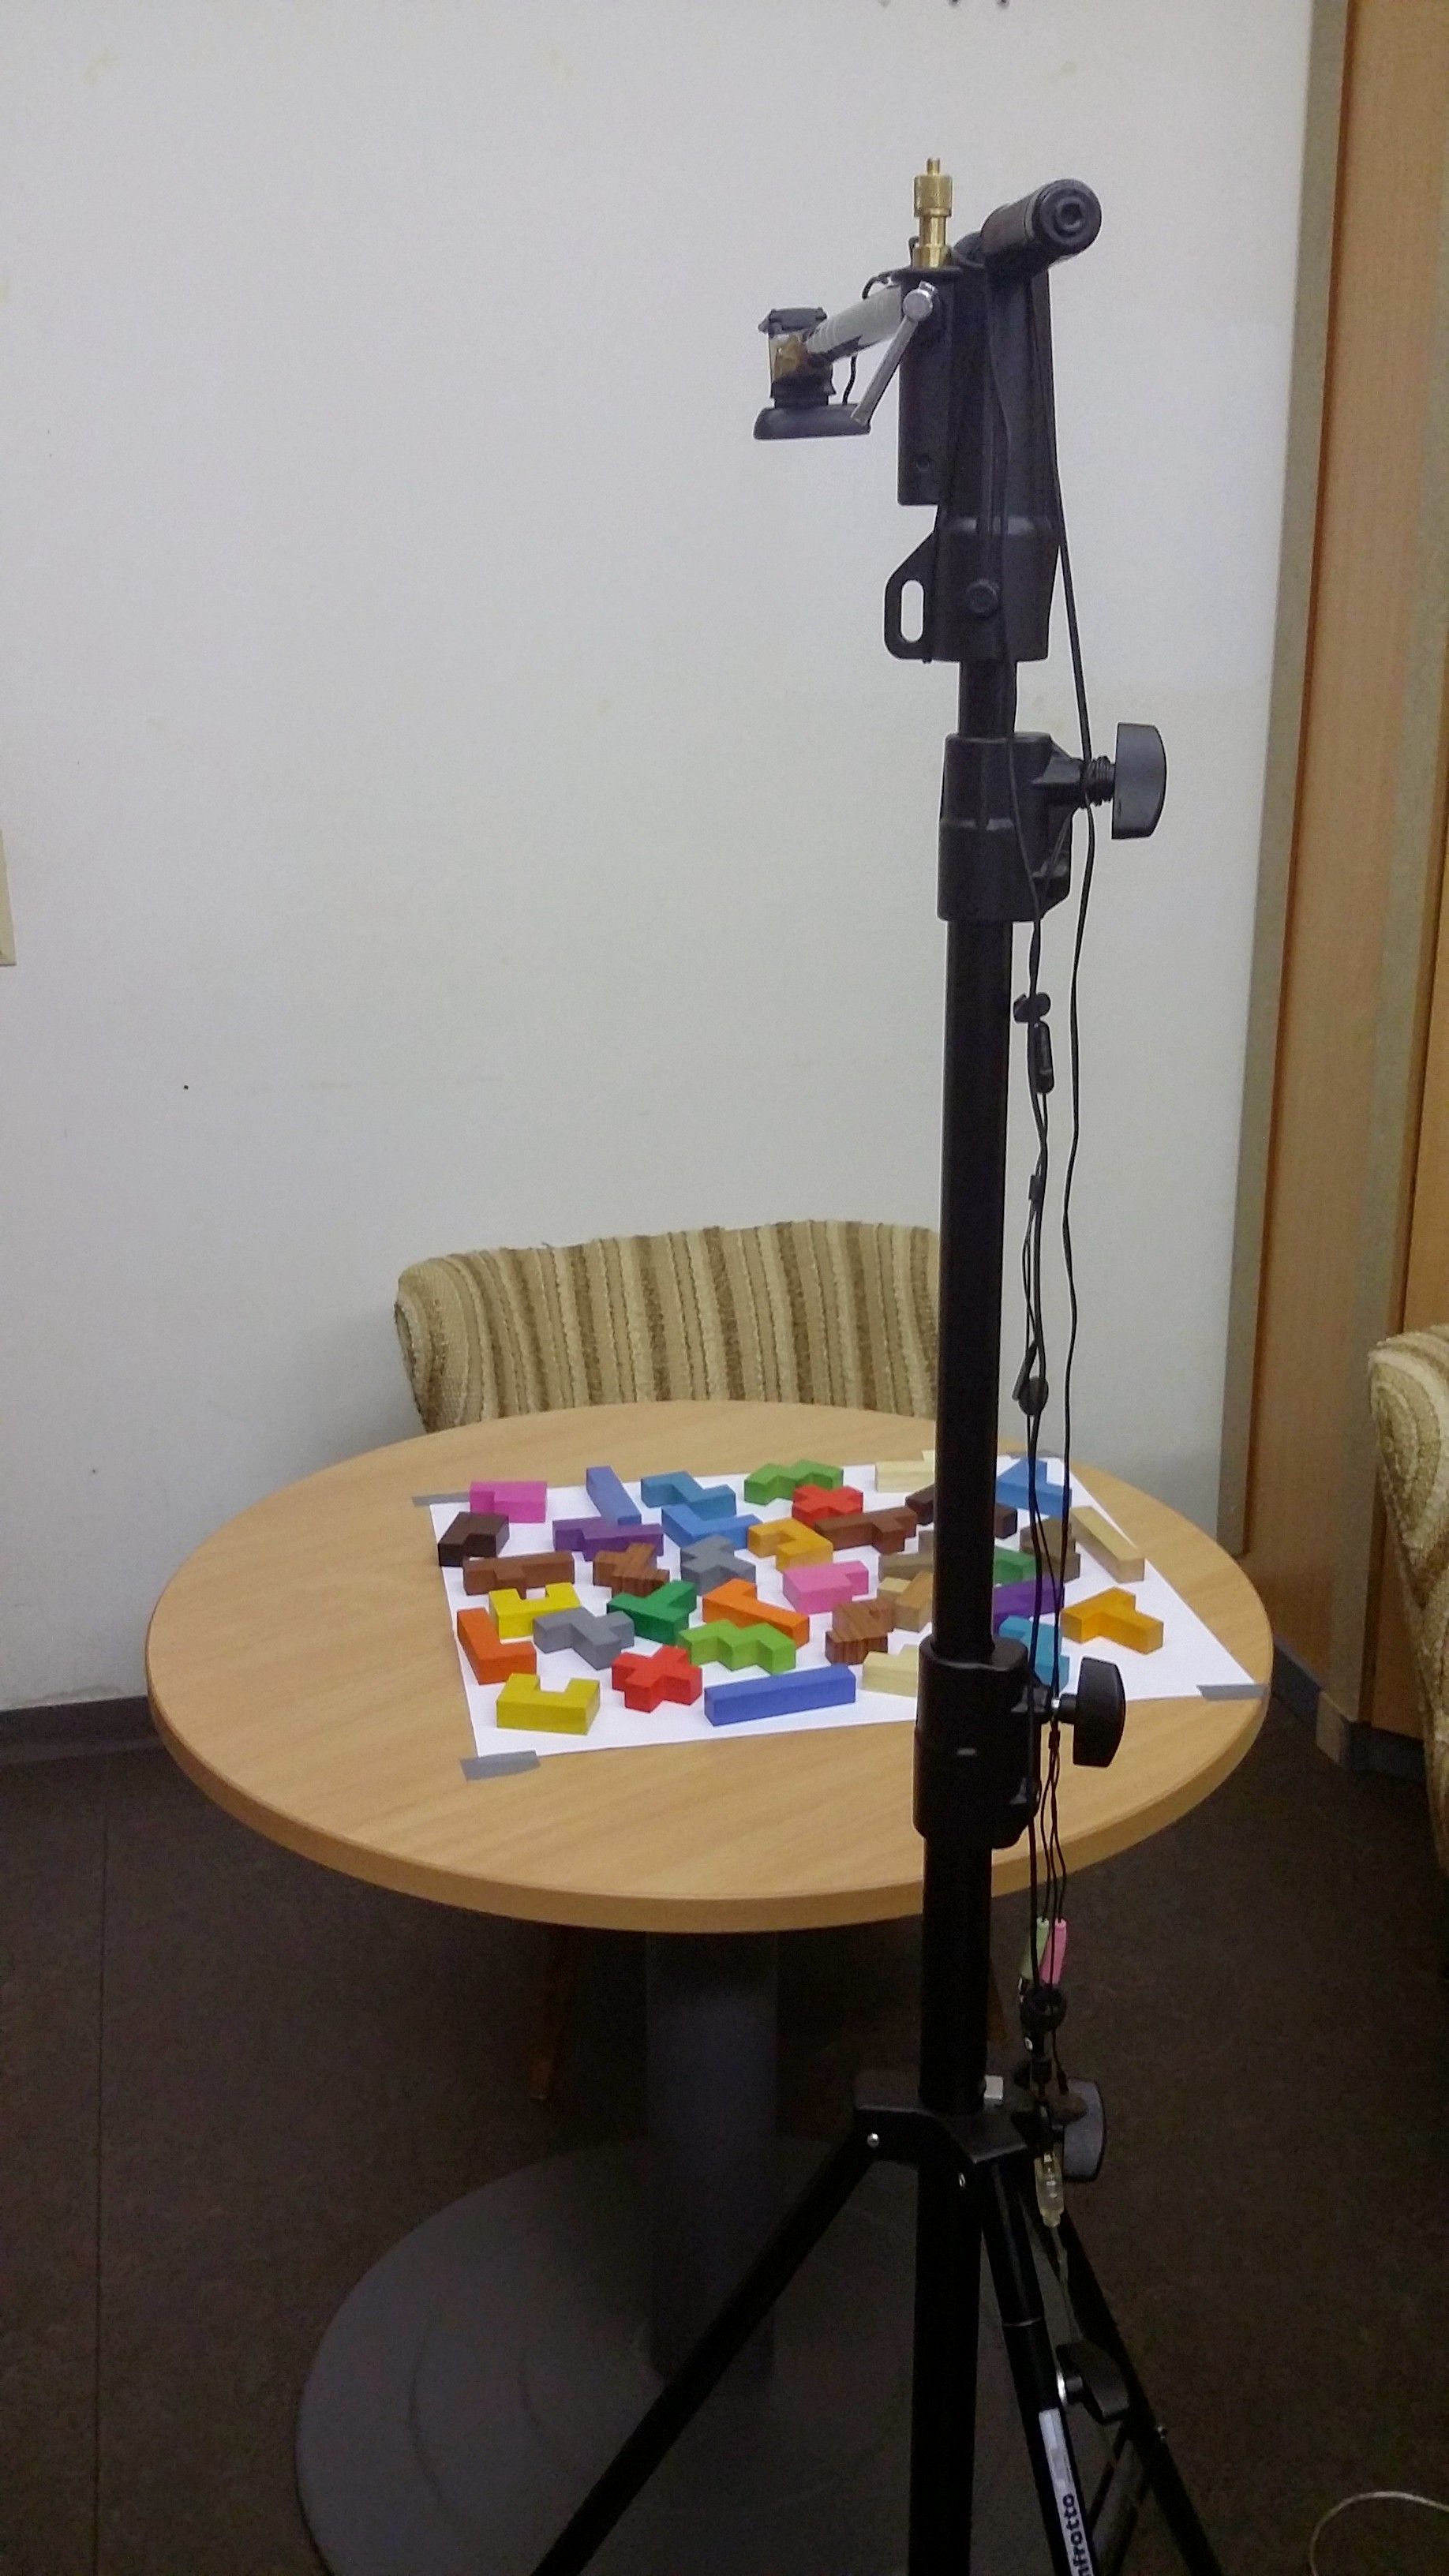
\includegraphics[width=0.5\textwidth]{takecvsetup.jpg}	
      \caption{Layout: table with pento objects, participant sits in front of it in a seat, a camera is above the table oriented in the same direction as the participant's viewpoint.\label{layout}}
\end{figure}

\section{Task}

The overall goal (like the TAKE Apr13 data) is to collect as many episodes of \textsc{re}s as possible in the time the participant interacts with our system (i.e., the wizard). An episode begins when a small screen shows an overlay of the Pentomino objects on the table. One object is then visibly selected by a green outline around the object's contour (with an optional landmark object). The participant is then to produce a \textsc{re} sufficient that the wizard can resolve the object.

We hope that it will be mostly self-annotating. That is, each episode will be easily segmented into a snapshot of the scene, the target and potential landmark. 

\section{Procedure}

\begin{figure}[ht]
\begin{minipage}{0.3\linewidth} 
\centering
      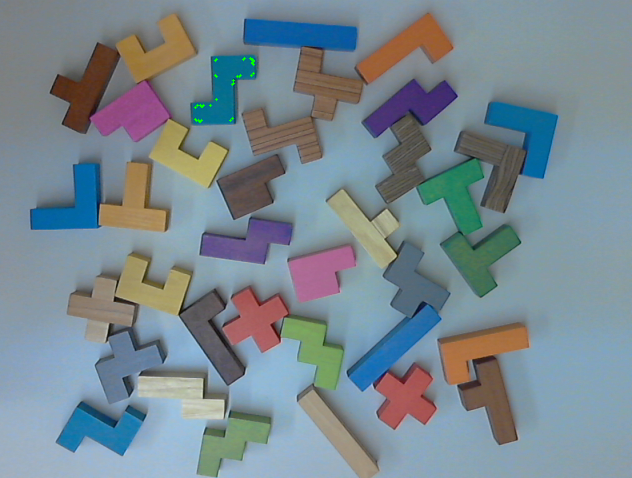
\includegraphics[width=1.0\textwidth]{targetonly.png}	
      \caption{Example target only (in green).\label{fig1}}
\end{minipage}
\hspace{0.25cm}
\begin{minipage}{0.3\linewidth} 
\centering
      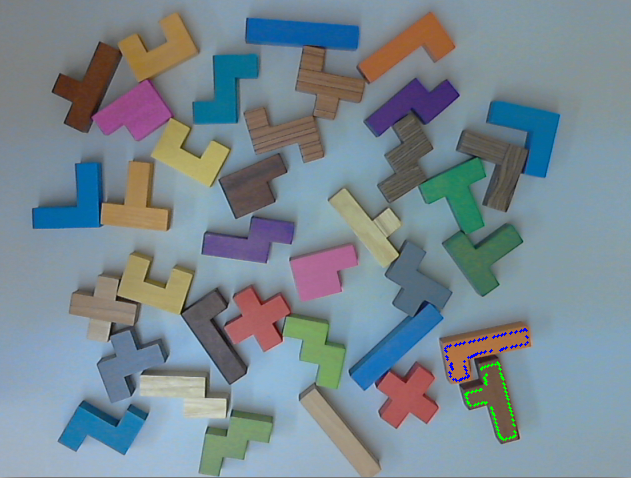
\includegraphics[width=1.0\textwidth]{relative.png}	
      \caption{Example target (in green) with landmark (in blue)\label{fig2}}
\end{minipage}
\hspace{0.25cm}
\begin{minipage}{0.3\linewidth} 
\centering
      
\includegraphics[width=1.0\textwidth]{shuffle.png}	
      \caption{Example signal for reshuffling.\label{fig3}}
\end{minipage}
\end{figure}

\paragraph{Before Task} Participants are to be brought into the lab and seated in front of a table with 36 pento objects on it in a marked area of the table. After signing the form and assuring agreement, they are to be explained the task. 

\paragraph{Explanation to Participant} In front of you is a table with objects of various shapes and colors on it. The screen in front of you shows those same shapes. When you see a green outline highlighting a target object, you are to find that object on the table and identify that object such that a person sitting next to you would know what object you are talking about (Figure \ref{fig1}). You can identify objects in any way you want (e.g., use color, shape, side of the table, what object is near it, etc.). However, if you also see a blue highlighted object near the target object, we ask that you identify the target by using that as a reference point (e.g., you are next to the table). We ask that you only use speech to identify to the object, please don't point to or pick up the object. The system will attempt to determine which object you described. If it is successful, then  a new target will be selected and the process will repeat. If it is not successful, a tone will sound, then it will select a new target and the process will repeat. We ask that you identify as many targets in the alloted time as possible, but please make sure the descriptions can uniquely identify the target.

At various times, a message ``Please Shuffle'' will appear on the screen (Figure \ref{fig3}). When that happens, please randomly move the objects around, but please be sure that all of the objects remain on the white area when you are done shuffling and that there are small gaps of space between the objects. After you are done shuffling, the message will disappear and a new target object will be selected as before.

\paragraph{After Task} The participant is to be thanked and paid the agreed amount. 


\section{Software}

We will be using OpenCV for object detection, using Livia Dia's python scripts to randomly select the target and landmark objects. OpenCV provides the ability to make multiple windows, so we can use that directly to create the wizard and the participant windows. 

We will also record the audio using a screen recording software with a timestamp. If this is done on a different computer, we will sync the audio by playing a succession of beeps at the beginning of the experiment and writing the time when that beep occured in a text file.

\paragraph{To be logged} 

Each episode will have the following information logged in a folder named for the episode id:

\begin{itemize}
 \item a png snapshot of the setting (what the wizard sees)
 \item a png snapshot of what the participant see (the setting with the target/landmark outlines)
 \item an ann.txt file which contains the (id,x,y) information for the target and landmark, if chosen
 \item a setting.xml file which contains the features of each segmented object
 \item a flagged.txt file is copied into the folder if the wizard explicitely flags the episode, or if the wizard clicks on the wrong objbect, in which case the x,y coordinates of the mouse click are written to the flagged.txt file
 \item a timestamps.txt file gives the start and end timestamps of the episode only if the episode finished by a mouse click (either correct or incorrect) by the wizard
\end{itemize}

We will do ASR after the experiment is complete. 


\end{document}
